\documentclass[letter,12pt]{article}
\usepackage[letterpaper,right=1in,left=1in,top=1in,bottom=1in]{geometry}
\usepackage{setspace}

\usepackage[utf8]{inputenc}   % allows input of special characters from keyboard (input encoding)
\usepackage[T1]{fontenc}      % what fonts to use when printing characters       (output encoding)
\usepackage{amsmath}          % facilitates writing math formulas and improves the typographical quality of their output
\usepackage[hyphens]{url}     % adds line breaks to long urls
\usepackage[pdftex]{graphicx} % enhanced support for graphics
\usepackage{tikz}             % Easier syntax to draw pgf files (invokes pgf automatically)
\usetikzlibrary{arrows}

\usepackage{mathptmx}           % set font type to Times
\usepackage[scaled=.90]{helvet} % set font type to Times (Helvetica for some special characters)
\usepackage{courier}            % set font type to Times (Courier for other special characters)

\usepackage[longnamesfirst, sort]{natbib}\bibpunct[]{(}{)}{,}{a}{}{;} % handles biblio and references 

\usepackage{rotating}         % sideway tables and figures that take a full page
\usepackage{caption}          % allows multipage figures and tables with same caption (\ContinuedFloat)

\usepackage{dcolumn}          % needed for apsrtable and stargazer tables from R to compile
\usepackage{arydshln}         % dashed lines in tables (hdashline, cdashline{3-4}, 
                              %see http://tex.stackexchange.com/questions/20140/can-a-table-include-a-horizontal-dashed-line)
                              % must be loaded AFTER dcolumn, 
                              %see http://tex.stackexchange.com/questions/12672/which-tabular-packages-do-which-tasks-and-which-packages-conflict


\newcommand{\mc}{\multicolumn}

%% TO ADD NOTES IN TEXT, PUT % BEFORE THE ONE YOU WANT DISABLED
\usepackage[disable]{todonotes}                            % no show
%\usepackage[colorinlistoftodos, textsize=small]{todonotes} % show notes
\newcommand{\emm}[1]{\todo[color=red!15, inline]{\textbf{Eric:} #1}}

%% \usepackage{xr} % allows cross-ref to other file
%% \externaldocument{urge15appendix}

%% %for submission: sends figs, tables, and footnotes to last pages
%% \RequirePackage[nomarkers,nolists]{endfloat}     % sends tables and figures to the end
%% \RequirePackage{endnotes}                        % turns fn into endnotes; place \listofendnotes where you want 
%%                                                  %the endnotes to appear (it must be after the last endnote).
%% \let\footnote=\endnote
%% \newcommand{\listofendnotes}{
%%    \begingroup
%%    \parindent 0pt
%%    \parskip 2ex
%%    \def\enotesize{\normalsize}
%%    \theendnotes
%%    \endgroup
%% }

%% % for submission: drop page numbers when producing title page
%% \pagenumbering{gobble} % Remove page numbers (and reset to 1)
%% \pagenumbering{arabic}% Arabic page numbers (and reset to 1)


\setcitestyle{citesep={;}}

\begin{document}

\title{Incumbency advantage upon removal of single-term limits: Mexican municipal elections}
\author{Eric Magar \\ ITAM, Mexico City
}
\date{\today}
\maketitle

% \newpage

\begin{abstract}
\noindent En route
%% \newline
%% \newline
%% \textbf{Keywords}: Separation of Powers, Urgency Prerrogatives, Fast Track Authority, Legislative Process, Latin America, Chile
\end{abstract}

% \newpage

%\doublespacing

\section{Introduction}

\noindent En route

\section{Reform, consequences}

2014 reform surprising removal of term limits. Adopted in 1934, cornerstone of partisan centralization of power under the PRI. Removed immediate reelection at all levels.

PAN placed removal among its requests, as was standard. Unlike the past, when left and PRI would veto, it was adopted along other changes.

Federal deputies can reelect for up to four consecutive three-year terms, senators for two consecutive six-year terms. Fearing that members of Congress might gain too much independence from party leaders, reformers retained some control: incumbents must be renominated by the same party in whose ticket they originally ran. Elaborate. 

Kick-off in the 2021 mid-term election.

At subnational level, reformers left some discretion to state legislatures. State law-makers: either 2-, 3-, or 4-term limits. For municipal officers single- or 2-term limits. Two states only retained single-term limits for municipal presidents, Hidalgo and Veracruz. Unelected municipal officers in Oaxaca's \emph{usos y costumbres} Party clause mandatory. Variable election calendars: incumbents on the ballot progressively. 

Figure \ref{F:horizons} reports relative frequencies of incumbents with shifting electoral horizons since the reform. Each vertical bar accounts for all municipalities with elected officeholders---a handful of new municipalities were carved out in the period, so column totals vary between 2,016 and 2,039. Gray segments include municipalities in Hidalgo and Veracruz, states that retained single term limits, as municipalities nationwide did before 2014. Non-reformers account for nearly 15 percent of yearly observations. The first batch of returning incumbents arrived in 2018, in darker green segments. A total of 273 municipal presidents from 17 states secured reelection for a consecutive term that year, 12 more joining them in 2019. Together these account for 14 percent of observed municipalities, or almost 20 percent when population-weighted. The inaugural proportion is remarkable, the 2018 races concurred with a presidential race won by a landslide that, we will see, probably depressed reelection rates. 

Two other patterns stand out. Term-limited municipal officers, in light green, have decreased gradually but steadily---from about 35 percent in 2015 to less than 5 percent in 2018. Unlike the gray segments, these incumbents remain ineligible for consecutive reelection due to reforms coming into force further down in time. 

Freshmen elected in 2015, representing nearly 50 percent of municipal officers, had a very different perspective from their predecessors, as they were not barred from running again at the end of the term.  

Other post-2014 incumbents, in light purple, remained term-limited due to reforms coming into force further down in time. This block shrank progressively from about one-third of municipalities in 2015 to less than 5 percent in 2018. By 2021, only returning incumbents will be term limited. 

\begin{figure}
  \centering
  \includegraphics[width=.8\columnwidth]{../graph/horizon-yrs.pdf} \\
  \caption{Extending the electoral horizons of municipal incumbents. Columns classify $N \approx 2,030$ municipalities according to the yearly reelection status of elected officeholders (430 municipalities with unelected indigenous governments are excluded).}\label{F:horizons}
\end{figure}
eric  x

Members of Congress can be reelected for up to 12 consecutive years. With 3-year terms, 

Term limits sever the personalized electoral connection, collective reputation only without the personal element.

See \citet{cain.etal.1987} for argumentation.

\section{A hypothesis perhaps}

\begin{description}
  \item [Hypothesis 1:] Presidents are more likely to fast-track bills when the committee chair with jurisdiction over the bill  belongs to the president's party than otherwise.
\end{description}

\section{Incumbents running v.\ open seats}


\begin{table}
  \caption{Success and failure with and without incumbent running}
  \begin{tabular}{l|cccc|cccc}
         &   \mc{4}{c|}{incumbent on the ballot}   &      \mc{4}{c}{open seat}           \\
In party & \%won   & \%lost   &   sum   &     (N)  & \%won  & \%lost &   sum   &      (N)\\ \hline
PAN      &   66    &   34     &   100   &   (121)  &   39   &   61   &   100   &   (1663)\\
PRI      &   49    &   51     &   100   &   (219)  &   50   &   50   &   100   &   (3546)\\
PRD      &   55    &   45     &   100   &    (88)  &   39   &   61   &   100   &   (1082)\\
Morena   &  100    &    0     &   100   &     (8)  &   88   &   12   &   100   &     (18)\\
Other    &   45    &   55     &   100   &    (99)  &   25   &   75   &   100   &    (631)\\ \hline
Total    &   54    &   46     &   100   &   (535)  &   44   &   56   &   100   &   (6940)\\
  \end{tabular}
\end{table}

\begin{tabular}{lcccccccc}
         &   \mc{4}{c}{incumbent on the ballot}    &      \mc{4}{c}{open seat, party}   \\
In party &   won   &   lost   &   sum   &   (N)    &   won  &   lost &   sum   &   (N)\\
left     &   58    &   42     &   100   &   (96)   &   39   &   61   &   100   &   (1100)\\
\end{tabular}

\section{Regression model}

% Table created by stargazer v.5.2.2 by Marek Hlavac, Harvard University. E-mail: hlavac at fas.harvard.edu
% Date and time: Tue, Sep 29, 2020 - 05:17:38 PM
% Requires LaTeX packages: dcolumn 
\begin{table}[!htbp] \centering 
  \caption{} 
  \label{} 
\begin{tabular}{@{\extracolsep{5pt}}lD{.}{.}{-3} D{.}{.}{-3} D{.}{.}{-3} } 
\\[-1.8ex]\hline 
\hline \\[-1.8ex] 
 & \multicolumn{3}{c}{\textit{Dependent variable:}} \\ 
\cline{2-4} 
\\[-1.8ex] & \multicolumn{3}{c}{Residual} \\ 
 & \multicolumn{1}{c}{PAN} & \multicolumn{1}{c}{PRI} & \multicolumn{1}{c}{Left} \\ 
\\[-1.8ex] & \multicolumn{1}{c}{(1)} & \multicolumn{1}{c}{(2)} & \multicolumn{1}{c}{(3)}\\ 
\hline \\[-1.8ex] 
 vote share (lagged) & -0.187^{***} & -0.035^{***} & -0.339^{***} \\ 
  & (0.011) & (0.013) & (0.013) \\ 
  & & & \\ 
 party incumbent & 0.224^{***} & 0.171^{***} & 0.165^{***} \\ 
  & (0.013) & (0.014) & (0.018) \\ 
  & & & \\ 
 other-party incumbent & -0.021^{**} & -0.011 & 0.005 \\ 
  & (0.010) & (0.009) & (0.010) \\ 
  & & & \\ 
 party open seat & 0.162^{***} & 0.124^{***} & 0.130^{***} \\ 
  & (0.004) & (0.004) & (0.005) \\ 
  & & & \\ 
 governor & -0.009^{*} & 0.028^{***} & 0.008 \\ 
  & (0.005) & (0.004) & (0.006) \\ 
  & & & \\ 
 population (10k) & 0.002 & 0.002^{**} & 0.006^{***} \\ 
  & (0.001) & (0.001) & (0.001) \\ 
  & & & \\ 
 elevation (pop. weigthed) & -0.003 & -0.00005 & -0.031^{***} \\ 
  & (0.003) & (0.003) & (0.003) \\ 
  & & & \\ 
 sd.elev & -0.143^{***} & -0.038 & -0.080^{**} \\ 
  & (0.034) & (0.031) & (0.035) \\ 
  & & & \\ 
 post reform & 0.085^{***} & -0.156^{***} & 0.047^{***} \\ 
  & (0.005) & (0.005) & (0.006) \\ 
  & & & \\ 
 elev x sd.elev & 0.105^{***} & -0.017 & 0.085^{***} \\ 
  & (0.024) & (0.022) & (0.025) \\ 
  & & & \\ 
 Intercept & -0.041^{***} & -0.036^{***} & -0.062^{***} \\ 
  & (0.005) & (0.007) & (0.004) \\ 
  & & & \\ 
\hline \\[-1.8ex] 
Observations & \multicolumn{1}{c}{8,314} & \multicolumn{1}{c}{8,314} & \multicolumn{1}{c}{8,314} \\ 
R$^{2}$ & \multicolumn{1}{c}{0.213} & \multicolumn{1}{c}{0.293} & \multicolumn{1}{c}{0.183} \\ 
%Adjusted R$^{2}$ & \multicolumn{1}{c}{0.212} & \multicolumn{1}{c}{0.292} & \multicolumn{1}{c}{0.182} \\ 
Residual Std. Error (df = 8303) & \multicolumn{1}{c}{0.163} & \multicolumn{1}{c}{0.152} & \multicolumn{1}{c}{0.169} \\ 
F Statistic (df = 10; 8303) & \multicolumn{1}{c}{225.2$^{***}$} & \multicolumn{1}{c}{344.3$^{***}$} & \multicolumn{1}{c}{185.6$^{***}$} \\ 
\hline 
\hline \\[-1.8ex] 
\textit{Note:}  & \multicolumn{3}{r}{$^{*}$p$<$0.1; $^{**}$p$<$0.05; $^{***}$p$<$0.01} \\ 
\end{tabular} 
\end{table} 


\section{Discussion}

\begin{figure}
  \centering
    \caption{Population-weigthed altitude deviations in municipalities}\label{F:avgMg}
    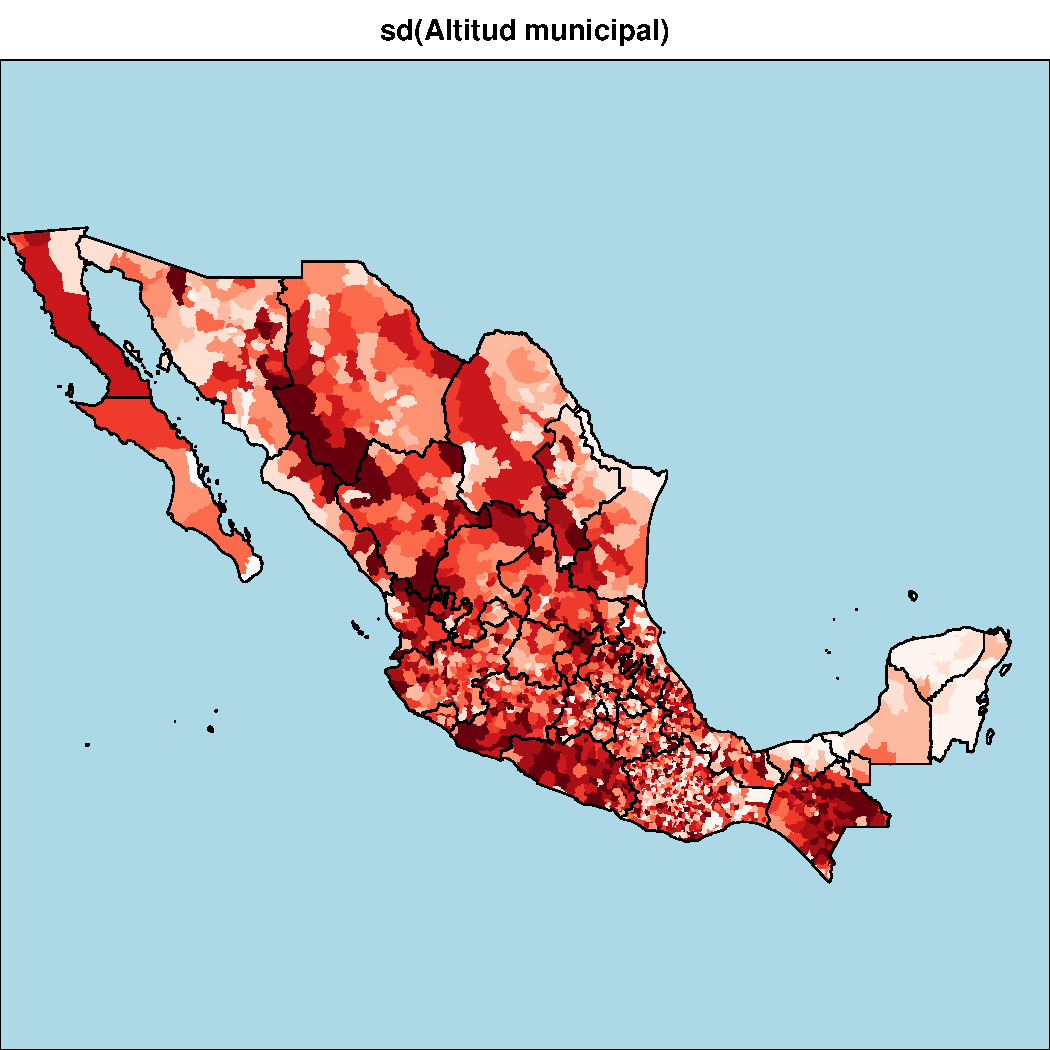
\includegraphics[width=.8\columnwidth]{../graph/map.png}
\end{figure}


\section*{Acknowledgements}
The author received financial support from the Asociaci\'on Mexicana de Cultura \textsc{a.c.}. He is responsible for mistakes and shortcomings in the study.

%% \listofendnotes

\bibliographystyle{apsr}
%\bibliography{../bib/magar}
\bibliography{/home/eric/Dropbox/mydocs/magar}

\end{document}

